\chapter{Vassiliev invariants and chord diagrams}
\label{ch:vassiliev-invariants-and-chord-diagrams}

\lettrine{\libertineInitialGlyph{V}}{assiliev} invariants are sophisticated to define in terms of the space of knots from the introduction, but the axiomatic definition of Birman-Lin \cite{knot-polynomials-and-vassilievs-invariants} is much simpler. The definition also illustrates an analogy made by Bar-Natan \cite{on-the-vassiliev-knot-invariants} in which Vassiliev invariants are ``polynomial invariants''. This is not meant in the sense that Vassiliev invariants take values in a polynomial ring (like say, the Jones polynomial), but rather that Vassiliev invariants have special properties not shared by all invariants, just as polynomial functions have special properties not shared by all functions.

\section{Singular knots}
\label{sec:singular-knots}

\begin{definition}
	A \textbf{singular knot} is an immersion of \(S^{1}\) into \(\R^{3}\) which fails to be an embedding at finitely many singularities, and where the singularities are all double-points of transverse intersection. When a singular knot has \(m\) such singularities, we call it \textbf{\(m\)-singular}.
\end{definition}

\begin{remark}
	\label{rem:other-singularities}
	Immersions with other types of singularities, are excluded from this definition, so the word ``singular'' in ``singular knot'' refers specifically to double point singularities. In particular immersions with
	\begin{enumerate}
		\item triple points
		\item points with vanishing derivative
	\end{enumerate}
	are excluded from the definition.
\end{remark}


A singular knot with one double point is very close to two other knots. In one, the double point is replaced by a positive crosing, and in the other a negative crossing.
If the conditions are right, we can extend a knot invariant to an invariant of singular knots by a procedure analagous to taking its derivative.
\begin{definition}
	\label{def:derivative}
	The \textbf{derivative} \(\delta\) of a differentiable \(m\)-singular knot invariant \(f\) is an \((m + 1)\)-singular knot invariant
	\[\delta f \left( \double \right) = f \left( \poscross \right) - f\left( \negcross \right).\]
\end{definition}

What are the conditions? For this to be a well-defined operation, it mustn't matter which double point we choose. % TODO: (Zsuzsi) I would only use a definition environment when you're ready to be precise and well defined. Here, we don't know yet what differentiable means, so I would save the definition environment for later (swap the two definitions).
% TODO (Damian) I'll think about this! My initial thought is that it's not too bad since differentiable is really close after, and since I disliked the other order.
%TODO (Zsuzsi) I still think this will annoy at least a significant subset of potential readers. You could start with an informal definition of the derivateive (ie not in an environment), then define differentiable, followed by the fornal definition of the derivaltive.

\begin{definition}
	\label{def:differentiable-invariant}
	An invariant \(f\) of \(m\)-singular knots is \textbf{differentiable} if
	\begin{equation}
		\label{eq:diff}
		\tag{\diff}
		f \left( \poscross \ \double \right) - f\left( \negcross \ \double \right) = f \left( \double \ \poscross \right) - f\left( \double \ \negcross \right).
	\end{equation}
\end{definition}

If an invariant of \(m\)-singular knots is differentiable, so is its derivative, so it can be extended to any number of double points.

Rather than thinking about functions on knots satisfying certain relations, the modern view of this subject takes the philosophy of imposing relations on the objects directly. 

\begin{definition}
	\label{def:differentiable-knot}
	Define \(\mathcal{K}_{m} = \operatorname{span}(\{m\text{-singular knots}\})\) (taken over \(\mathbb{Q}\))
    modulo the following boundary relation (also known as a codifferentiability relation):
	\begin{equation}
		\label{eq:codiff}
		\tag{\codiff}
		\poscross \ \double - \negcross \ \double = \double \ \poscross - \double \ \negcross.
	\end{equation}
	From now on, we will refer to elements \(\mathcal{K}_{m}\) as \(m\)\textbf{-singular knots}, i.e. the \ref{eq:codiff} relation will be implicitly assumed.
\end{definition}

\begin{definition}
	\label{def:boundary}
	The \textbf{boundary} operation is the map \(\partial : \mathcal{K}_{m} \to \mathcal{K}_{m - 1}\) defined by
	\[ \double \longmapsto \poscross - \negcross .\]
\end{definition}

\begin{remark}
	The derivative operation and the \ref{eq:diff} relation are dual to the boundary operation and the \ref{eq:codiff} relation. For example, a differentiable invariant of knots is the same as an invariant of knots in \(\mathcal{K}_{m}\).
\end{remark}

Any knot invariant, \(f\) can be extended to an invariant \(f^{(m)}\) of \(m\)-singular knots by the Vassiliev skein relation 
\[f^{(0)} = f\]
and
\[f^{(m + 1)}\left(\double\right) = f^{(m)}\left(\poscross\right) - f^{(m)}\left(\negcross\right).\]
Often, we omit the superscript and write
\[f\left(\double\right) = f\left(\poscross\right) - f\left(\negcross\right).\]

The Vassiliev skein relation extends a knot via its derivative, or chooses a value on \((m + 1)\)-singular knots to agree with the difference of values on its boundary.



\begin{definitions}
	\label{def:vassiliev-invariant}
	\begin{enumerate}
		\item A knot invariant \(V\) is a \textbf{Vassiliev invariant} of order (or type) \(m\) if when extended to singular knots via the Vassiliev skein relation,
		\[V\biggl( \underbrace{\double \cdots \double}_{{\scriptscriptstyle m + 1}} \biggr) = 0.\]
	\item The \textbf{order} of a Vassiliev invariant \(V\) is the highest \(m\) such that \(V\) is a Vassiliev invariant of order \(m\). (That is, the order of a Vassiliev invariant is the most double points a knot \(K\) can have without \(V(K)\) having to vanish).
	\end{enumerate}
\end{definitions}

\begin{remark}
	In other words, Vassiliev invariants of order \(m\) are those that vanish after \(m + 1\) derivatives, just like degree \(m\) polynomials.
\end{remark}

\section{Integration and the fundamental theorem}
\label{sec:integration-and-the-fundamental-theorem}

To help see the bird's eye view, and following \cite{integration-of-singular-braid-invariants}, we phrase this in terms of an integration theory.
%TODO (Zsuzsi) Since this is the first sentence of a section, I would replace "this" with what "this" is referring to.


\begin{definition}
	An \textbf{integration theory} \((\mathcal{O}_{\star}, \partial_{\star})\) is a sequence
	% https://q.uiver.app/#q=WzAsNixbMSwwLCJcXG1hdGhjYWx7T31fe219Il0sWzAsMCwiXFxjZG90cyJdLFsyLDAsIlxcbWF0aGNhbHtPfV97bSAtIDF9Il0sWzMsMCwiXFxjZG90cyJdLFs0LDAsIlxcbWF0aGNhbHtPfV97MX0iXSxbNSwwLCJcXG1hdGhjYWx7T31fezB9Il0sWzEsMCwiXFxwYXJ0aWFsIl0sWzAsMiwiXFxwYXJ0aWFsIl0sWzIsMywiXFxwYXJ0aWFsIl0sWzMsNCwiXFxwYXJ0aWFsIl0sWzQsNSwiXFxwYXJ0aWFsIl1d
	\[\begin{tikzcd}
		\cdots & {\mathcal{O}_{m}} & {\mathcal{O}_{m - 1}} & \cdots & {\mathcal{O}_{1}} & {\mathcal{O}_{0}}
		\arrow["\partial", from=1-1, to=1-2]
		\arrow["\partial", from=1-2, to=1-3]
		\arrow["\partial", from=1-3, to=1-4]
		\arrow["\partial", from=1-4, to=1-5]
		\arrow["\partial", from=1-5, to=1-6]
	\end{tikzcd}\]
	of abelian groups. In case we need to refer to a specific map, let \(\partial_{m}\) denote the map \(\partial\) whose domain is \(\mathcal{O}_{m}\). Note that we do not assume \(\partial^{2} = 0\).
\end{definition}

The group \(\mathcal{O}_{0}\) is typically free abelian, and in our case this is the primary object we want to study. The groups \(\mathcal{O}_{m}\) are also typically free abelian groups, and can often be thought of as \(m\)-singular objects of some kind. The map \(\partial\) takes an \(m\)-singular object \(x\) to some combination of \((m - 1)\)-singular objects near \(x\).

By fixing an abelian group \(G\) and setting \(\mathcal{O}_{m}^{\ast} = \operatorname{Hom}(\mathcal{O}_{m}, G)\), we get the sequence
% https://q.uiver.app/#q=WzAsNixbMSwwLCJcXG1hdGhjYWx7T31fe219XntcXGFzdH0iXSxbMCwwLCJcXGNkb3RzIl0sWzIsMCwiXFxtYXRoY2Fse099X3ttIC0gMX1ee1xcYXN0fSJdLFszLDAsIlxcY2RvdHMiXSxbNCwwLCJcXG1hdGhjYWx7T31fezF9XntcXGFzdH0iXSxbNSwwLCJcXG1hdGhjYWx7T31fezB9XntcXGFzdH0iXSxbMCwxLCJcXGRlbHRhIiwyXSxbMiwwLCJcXGRlbHRhIiwyXSxbMywyLCJcXGRlbHRhIiwyXSxbNCwzLCJcXGRlbHRhIiwyXSxbNSw0LCJcXGRlbHRhIiwyXV0=
\[\begin{tikzcd}
	\cdots & {\mathcal{O}_{m}^{\ast}} & {\mathcal{O}_{m - 1}^{\ast}} & \cdots & {\mathcal{O}_{1}^{\ast}} & {\mathcal{O}_{0}^{\ast}}
	\arrow["\delta"', from=1-2, to=1-1]
	\arrow["\delta"', from=1-3, to=1-2]
	\arrow["\delta"', from=1-4, to=1-3]
	\arrow["\delta"', from=1-5, to=1-4]
	\arrow["\delta"', from=1-6, to=1-5]
\end{tikzcd}\]
where \(\delta_{m}\) is the transpose of \(\partial_{m}\). The maps \(\delta\) behave like derivatives: \(\delta(f)\) for \(f \in \mathcal{O}_{m}^{\ast}\) defines \(f\) on \(\mathcal{O}_{m + 1}^{\ast}\) as some combination of its values on ``close'' \(m\)-singular objects.

We wish to understand how to invert this process, namely:
%TODO (Zsuzsi) I would move the sentence above into the question environment.
\begin{questions}
	\label{qu:integration-theory}
	\begin{enumerate}
		\item When does a functional in \(\mathcal{O}^{\ast}_{m}\) ``integrate'' to a functional in \(\mathcal{O}^{\ast}_{m - 1}\)?
		\item Is the integral of a functional in \(\mathcal{O}_{m}^{\ast}\) uniquely defined, or are there choices to be made?
		\item When does such a functional integrate multiple times, in-particular when does it integrate \(m\) times into a functional in \(\mathcal{O}^{\ast}_{0}\), (i.e. a function on the non-singular objects)?
		\item If there are choices to be made in integration, do they affect whether the new functional is integrable again?
		\item Which functions on the non-singular objects \(\mathcal{O}_{0}\) are obtained by \(m\) consecutive integrations of functionals in \(\mathcal{O}_{m}^{\ast}\)?
	\end{enumerate}
\end{questions}
The following modules provide the tautological answers to the above questions in the general theory. %TODO (Zsuzsi) I would explain in what sense these are modules (under what action).
%TODO (Zsuzsi) I see what you're saying here with "tautological", though it's a bit intimidating to use that word when the way in which these are tautological answers is non-trivial. Maybe you can make it into a word joke by saying this here, rather then after the intimidation...
\begin{definitions}
	\label{def:integration-theory-modules}
	\begin{enumerate}
		\item The \textbf{primary obstructions to integration} are the module
			\[P\mathcal{O}_{m} = \ker{\partial_{m}}.\]
		\item The \textbf{constants of integration} are the module
			\[C\mathcal{O}_{m} = \mathcal{O}_{m} / \partial \mathcal{O}_{m + 1}.\]
		\item The \textbf{secondary obstructions to integration} are the module
			\[S\mathcal{O}_{m} = \ker{(\partial_{m + 1}\partial_{m})} / P\mathcal{O}_{m},\]
			and likewise the \textbf{order \(k\) obstructions to integration} are defined analagously.
		\item The \textbf{weights of integration} are the module
			\[W\mathcal{O}_{m} = C\mathcal{O}_{m} / \pi(P\mathcal{O}_{m})\]
			where \(\pi: \mathcal{O}_{m} \to C\mathcal{O}_{m}\) is the projection.
		\item The \textbf{finite type invariants} of order \(m\) are the module
			\[FT\mathcal{O}_{m} = \ker \delta^{m + 1},\]
			where \(\delta^{m + 1}\) denotes \(m + 1\) applications of \(\delta\) with appropriate indices, ending with \(\delta_{m}\).

	\end{enumerate}
\end{definitions}
It may not be entirely obvious how these definitons provide answers to the questions above. In the rest of this section we will see the truth of this in the case \(\mathcal{O}^{\star} = \mathcal{K}^{\star}\) 
%TODO (Zuzsi) $\mathcal{O}=\mathcak{K}$?
which provides good intuition for the general case.

Recall from the picture from the introduction 
%TODO Zsuzsi If you're referencing a figure, have the figure number (eventually)
that \(m\)-singular knots are components of the stratification of the space of knots of codimension \(m\).

\begin{definition}
	A \textbf{singular isotopy}, \(\Psi(t)\) of \(m\)-singular knots is a path in the union of the \(m\)-th and \((m + 1)\)-st strata such that the path only intersects the \((m + 1)\)st stratum transversally and finitely many times. The intersections \(\{\Psi_{s} : 1 \leq s \leq r\}\) of the path with the \((m + 1)\)st stratum are called the \textbf{singularities} of the singular isotopy. The \textbf{signs} \(\varepsilon_{s} = \varepsilon(s): \{s\} \to \{\pm 1\}\) of the singularities give the signs of the corresponding intersection.
\end{definition}

% TODO: Insert an image of a singular isotopy.

To rephrase the definitions in Section~\ref{sec:singular-knots}, in the integration theory \(\mathcal{O}^{\star} = \mathcal{K}^{\star}\), 
%TODO (Zuzsi) $\mathcal{O}=\mathcak{K}$?
differentiation constructs from an invariant \(Q\) of \(m\)-singular knots, an invariant \(Q'\) of \((m + 1)\)-singular knots such that along singular isotopies from \(k_{0}\) to \(k_{1}\),
\[Q(k_{0}) - Q(k_{1}) = \sum_{s = 1}^{r}\varepsilon_{s} Q'(\Psi_{s}).\]
Due to the boundary relation this is always well-defined.

Integration is to construct from an invariant \(P\) of \((m + 1)\)-singular knots an invariant \(Q\) of \(m\)-singular knot such that
\[Q(k_{0}) - Q(k_{1}) = \sum_{s = 1}^{r}\varepsilon_{s} P(\Psi_{s}),\]
in which case we write \(P = Q'\). This is like a ``path-integral'' along a singular isotopy. For this to be well-defined, \(P\) needs to be path-independent. Equivalently, all integrals along closed paths (where \(k_{0} = k_{1}\)) must vanish. In particular, recall from Remark \ref{rem:other-singularities} that triple points and points with vanishing derivative are excluded from all levels of the stratification, leaving ``holes'' in the strata. The vanishing of integrals along singular isotopies around such holes give rise to the following relations, and satisfying these are necessary conditions for \(P\) to integrate:

\begin{definitions}
	\begin{enumerate}
		\item The following closed singular isotopy around a triple point:
			\begin{center}
				\def\svgwidth{0.6\columnwidth}
				\input{graphics/triple_point_singular_isotopy.pdf_tex}
			\end{center}
		gives rise to the \textbf{topological four-term relation}
			\begin{equation}
				\label{eq:topological-four-term}
				\tag{\tft}
				f\left( \tftsouth \right)
				-
				f\left( \tfteast \right)
				-
				f\left( \tftnorth \right)
				+
				f\left( \tftwest \right)
				= 0.
			\end{equation}
		\item The closed singular isotopy
			\begin{center}
				\def\svgwidth{0.6\columnwidth}
				\input{graphics/vanishing_derivative_singular_isotopy.pdf_tex}
			\end{center}
		around a point with a vanishing derivative gives rise to the \textbf{topological one-term relation}
			\begin{equation}
				\label{eq:topological-one-term}
				\tag{\tot}
				f\left( \totgraphic \right) = 0.
			\end{equation}
	\end{enumerate}
\end{definitions}

The necessity of the above relations for an invariant of \(m\)-singular knots to integrate is equivalent to the assertion that
\[
	\tftsouth
	\ - \
	\tfteast
	\ - \
	\tftnorth
	\ + \
	\tftwest
	\quad \text{and} \quad
	\totgraphic
\]
are in \(P\mathcal{K}_{m} = \ker \partial_{m}\). Let us denote arbitrary such singular knots \(\tftterm\) and \(\totterm\). 
%TODO (Zsuzsi) I have trouble parsing the last sentence... The set of all (linear combinations of) such singular knots? Any particular singular knot participating in these relations?

This raises the question of whether we have found all primary obstructions. Do \(\tftterm\) and \(\totterm\) span \(\ker \partial\)?

\begin{theorem}[Stanford \cite{finite-type-invariants-of-knots-links-and-graphs}]
	\label{thm:stanford-integrates-once}
	An invariant \(f\) of \(m\)-singular knots integrates to an invariant of \(m - 1\)-singular knots if and only if it satisfies \textup{\ref{eq:topological-four-term}} and \textup{\ref{eq:topological-one-term}}.
\end{theorem}

{\color{red}
ZSUZSI READ TO HERE}

\begin{proof}[sketch]
	% TODO: Fill out Stanford's integration homotopy proof
	\begin{mdframed}
		Let \(\gamma = \Psi(t)\) be a singular isotopy and let \(\Phi(\gamma)\) be the path integral along it. Construct a homotopy from \(\gamma\) to the constant singular isotopy in the stratification of knots with at least \(m - 1\) double points, and additional worse singularities. The only events to consider are codimension \(m + 2\) (why \(m + 2\)? is it to do with homotopy being "2"-dimensional?) events. They all change the \(\Phi(\gamma)\) by \(f(\tftterm)\) or \(f(\totterm)\) (or similar with \ref{eq:diff} relations, which we've said are implicit).

		Once the homotopy is complete, we are done as \(\Phi(\gamma_{\text{const}}) = 0\). On a down-to-earth level, why does this imply \(f\) can be integrated?
	\end{mdframed}
\end{proof}

In the order of Questions \ref{qu:integration-theory} and Definitions \ref{def:integration-theory-modules}, we ought to talk next about the secondary and further obstructions to integration. However, let us postpone this until after we have discussed constants of integration, which will be a more natural place.

The constants of integration comprise the information that is lost when integrating. In the case of knots, differentiating defines an invariant \(\delta f\) on \((m + 1)\)-singular knots as the difference of \(f\) on two neighbouring \(m\)-singular knots, but the value of the invariant on either of these \(m\)-singular knots is lost. When integrating, values on these can be chosen freely. Recall from Definition \ref{def:integration-theory-modules} (b) that \(C\mathcal{K}_{m} = \mathcal{K}_{m} / \partial \mathcal{K}_{m + 1}\). The difference of an \(m\)-singular knot and the same \(m\)-singular knot with one crossing changed is the image of some \((m + 1)\)-singular knot under \(\partial\). We see that constants of integration are singular knots which are blind to crossing changes, so the only data needed to describe them is the order in which the double points are traversed around the knot.

\begin{definitions}
	\label{def:chord-diagram}
	\begin{enumerate}
		\item A \textbf{chord diagram} of order \(m\) is an element of \(\mathcal{K}_{m} / \partial \mathcal{K}_{m + 1}\). This is equivalent to an oriented circle with a distinguished set of \(m\) pairs of points, considered up to orientation-preserving diffeomorphism of the circle. Chords are drawn between each pair of points. The vector space spanned by chord diagrams of order \(m\) is denoted \(\mathcal{D}_{m}\), so \(\mathcal{D}_{m} = C\mathcal{K}_{m}\).
		\item The \textbf{chord diagram of an \(m\)-singular knot \(K\)}, denoted \(\pi(K)\) is the chord diagram formed by the following process. Place \(2m\) points on an oriented circle, two for each singular point of \(K\). Traversing both \(K\) and the circle, label the points on the circle in the order in which the singular points of \(K\) are traversed. Each label is given twice, pairing up the \(2m\) points, forming \(\pi(K)\).
	\end{enumerate}
\end{definitions}

\begin{example}
	\[
		\includegraphics[width=0.14\textwidth, valign=c]{graphics/knot_9_33_singular.pdf}
		\quad \overset{\pi}{\longmapsto} \quad
		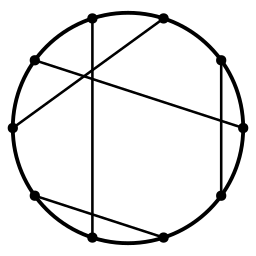
\includegraphics[width=0.13\textwidth, valign=c]{graphics/chord_diagram_of_knot_9_33_singular.pdf}
	\]
\end{example}

\begin{proposition}
	Suppose \(P\) is an integrable \(m\)-singular invariant with integral \(Q\). Let \(Q_{0}\) differ from \(Q\) by a function on chord diagrams, that is
	\[Q_{0}(k) = Q(k) + q(\pi(k))\]
	for \(q \in \mathcal{D}_{m}^{\ast}\)
	Then \(Q_{0}\) is also an integral of \(P\).
\end{proposition}

\begin{proof}
	The derivative of a function of chord diagrams is zero, as two knots which differ by a crossing change have the same chord diagram. Hence \(Q\) and \(Q_{0}\) have the same derivative: \(P\).
\end{proof}

\begin{remark}
	We defined a constant of integration as a set of objects (e.g. \(c \in \mathcal{D}_{m}\)) but perhaps it would have been more accurate to define it as a functional (e.g. \(q \in \mathcal{D}_{m}^{\ast}\)). After all the constant of integration on the real line is ``\(+ \ C\)'' rather than the set \(\{\ast\}\) with one object. There is no real risk of confusion, so let us be slightly loose and use the terminology for either.
\end{remark}

Since we are trying to integrate more than once, we might wish to know which constants of integration are themselves integrable.

\begin{definition}
	\label{def:weight-system}
	A \textbf{weight system} is an integrable \(w \in \mathcal{D}_{m}^{\ast}\).
\end{definition}

If we take the relations for a knot invariant to be integrable and project them into the space of chord diagrams, we get the following relations.

\begin{definition}
	\label{def:ft-ot-relations}
	\begin{enumerate}
		\item The \textbf{four-term relation} is the relation
			\begin{equation}
				\label{eq:4T}
				\tag{\ft}
				q\left(\ftsouth\right)
				- q\left(\fteast\right)
				- q\left(\ftnorth\right)
				+ q\left(\ftwest\right)
				= 0.
			\end{equation}

		\item The \textbf{one-term relation} is the relation
			\begin{equation}
				\label{eq:1T}
				\tag{\ot}
				q\left( \otgraphic \right) = 0.
			\end{equation}
	\end{enumerate}
\end{definition}

\begin{remark}
	Just like \ref{eq:topological-four-term} and \ref{eq:topological-one-term}, \ref{eq:4T} and \ref{eq:1T} are not individual relations, but kinds of relations. To satisfy them, \(q \in \mathcal{D}_{m}^{\ast}\) needs to satisfy them for all ways additional chords can be placed into the diagram to make a diagram of degree \(m\), so long as they don't go between the close chord-ends.
\end{remark}

\begin{proposition}
	A weight system is characterised as a constant of integration that satisfies \textup{\ref{eq:4T}} and \textup{\ref{eq:1T}}.
\end{proposition}
\begin{proof}
	A weight system defines an \(m\)-singular invariant that is also invariant under crossing change. To integrate it must satisfy \ref{eq:4T}  and \ref{eq:1T}. Since crossing changes are free, this is equivalent to satisfying the projection of \ref{eq:topological-four-term} and \ref{eq:topological-one-term} into chord diagrams.
\end{proof}

We return now to the secondary (and higher) obstructions. A general integral of on \(m\)-singular \(P\) is of the form
\[Q + q \circ \pi.\]
Since integration is linear, to be integrable again, both terms need to be integrable. The latter we have just seen as the condition that \(q\) is a weight system. A sufficient condition for the former to be integrable is that \(S\mathcal{K}_{m}\) vanishes. But this is a tautological statement of the general theory --- it doesn't mean much if we don't know what \(S\mathcal{K}_{m}\) is.

\begin{conjecture}
	\label{conj:strong-fundamental-theorem}
	An invariant of \(m\)-singular knots satisfying \textup{\ref{eq:topological-four-term}} and \textup{\ref{eq:topological-one-term}} integrates \(m\) times into a genuine knot invariant.
\end{conjecture}

\begin{remarks}
	\begin{enumerate}
		\item At first glance, this conjecture looks like it follows from Theorem~\ref{thm:stanford-integrates-once}. The point is that it may not be possible to choose the integral to again satisfy \(\ref{eq:topological-four-term}\) and \(\ref{eq:topological-one-term}\), which is what \(S\mathcal{K}\) measures.
		\item Computing \(S\mathcal{K}_{m}\) is dual to computing \(\ker \partial_{m + 1} \partial_{m} / \ker \partial_{m}\) (we saw a similar thing with the primary obstructions). Computing \(\ker \partial^{2}\) is the hard part --- it's not too hard to find some elements, but whether they form a spanning set is open.
		% TODO: Expand this out into a little interlude on graph cohomology?
		\item This conjecture is proven in certain cases. It holds the integration theory for braids \cite{integration-of-singular-braid-invariants}, and in a certain sense it's ``half''-proven for knots \cite{a-combinatorial-half-integration-from-weight-system-to-vassiliev-knot-invariant}. In Chapter \ref{ch:combinatorial-integration_of_weight_systems} we extend this to ``a little more than half''.
	\end{enumerate}
\end{remarks}

The finite type invariants in \(\mathcal{K}^{\star}\) are simply the Vassiliev invariants, as checked by a simple comparison between Definitions \ref{def:vassiliev-invariant} and \ref{def:integration-theory-modules}. In other words, Vassiliev invariants of order \(m\) are those which vanish on parts of the strata at and above some depth \(m + 1\).

If we restrict Conjecture \ref{conj:strong-fundamental-theorem} to Vassiliev invariants, then we get the following.

\begin{theorem}[Fundamental theorem of Vassiliev invariants]
	\label{thm:fundamental-theorem-of-vassiliev-invariants}
	Let \(v\) be an invariant of \(m\)-singular knots satsifying \textup{\ref{eq:topological-four-term}}, \textup{\ref{eq:topological-one-term}} and the additional condition that \(\delta^{k} v = 0\). Then \(v\) integrates \(m\) times into a genuine knot invariant (which is a Vassiliev invariant).
\end{theorem}

There are various proofs of the fundamental theorem. They are listed in \cite{the-fundamental-theorem-of-vassiliev-invariants}, and each proof is accompanied by a series of moral objections. To quote their introduction: ``Always the method is indirect and very complicated, and/or some a-priori unnatural choices have to be made''. To summarise their philosophy:

\begin{remark}
	We have the implication Conjecture \ref{conj:strong-fundamental-theorem} \(\implies\) Theorem \ref{thm:fundamental-theorem-of-vassiliev-invariants}, and this is actually realised in the theory of braids. It is mysterious that the fate of the slightly stronger conjecture which comes from taking natural topological approach to the fundamental theorem still remains unknown, and that there are grievances to be had with all known proofs.
\end{remark}

In the Section \ref{sec:chord-diagrams-and-the-universal-Vassiliev-invariant} we will look at equivalent formulation of the fundamental theorem, and then in Chapter \ref{ch:combinatorial-integration_of_weight_systems} we present some progress towards Conjecture \ref{conj:strong-fundamental-theorem}.

\section{The algebra of chord diagrams}
\label{sec:the-algebra-of-chord-diagrams}

\begin{mdframed}
	Scaffold for this chapter.

	\(\cdot\) Begin with the connected sum on plain knots (don't talk about modding by 1T 4T yet).
	
	\(\cdot\) This induces a connected sum on singular knots (define via commutative diagram).
	
	\(\cdot\) This nearly induces a conntected sum on chord diagrams... except need to mod out by 4T and 1T which we were gonna do anyway.
\end{mdframed}

There is also an interesting algebraic structure on the space of knots, \(\mathcal{K}_{0}\) which extends to chord diagrams.

\begin{definition}
	\label{def:connected-sum}
	The \textbf{connected sum} of two knots \(K_{1}\) and \(K_{2}\) is the knot obtained by removing a small arc from each of \(K_{1}\) and \(K_{2}\), then connecting the two embedded intervals into a single knot in an orientation-preserving way.

	\[
		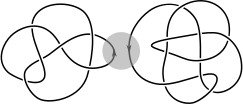
\includegraphics[width=0.37\textwidth, valign=c]{graphics/connected_sum_example_before.pdf}
		\quad
		\overset{\#}{\longmapsto}
		\quad
		\includegraphics[width=0.37\textwidth, valign=c]{graphics/connected_sum_example_after.pdf}
	\]
% TODO: Fix alpha layers being different in the above.

\end{definition}

This in not a-priori well-defined: we have not specified where along either \(K_{1}\) or \(K_{2}\) the small arc is to be removed. However, by a classical knot-theoretic argument, the result is independent of the choice.

\begin{proposition}
	The connected sum \(\#: \mathcal{K}_{0} \otimes \mathcal{K}_{0} \to \mathcal{K}_{0}\) forms a well-defined operation. It does not matter where along either knot the small arc was removed, the reslts are ambient-isotopic.
\end{proposition}

\begin{proof}
	We exhibit an ambient isotopy starting at \(K_{1} \# K_{2}\) where the small arc is removed from \(K_{1}\) as in the example above. The part of the connected sum coming from \(K_{2}\) is shrunk by ambient isotopy to an arbirarily small tubular neighbourhood of \(K_{1}\). \(K_{2}\) is then isotoped along \(K_{1}\), then reenlarged and isotoped back to its original position.
\end{proof}

The definition can be extended to singular knots.

\begin{definition}
	The \textbf{connected sum} of two singular knots is defined in the same way as the connected sum of two non-singular knots.
\end{definition}

\begin{mdframed}
	There's a slight problem here. The usual definition when singular knots are defined as linear combinations is by bilinear extension. This makes everything well-defined. However, for us, singular knots are literally singular knots. So the usual connected-sum-well-definedness argument fails because we can't move the small knot in a bubble through a double point.

	But perhaps we should expand our definition of singular isotopy to make this okay. Maybe a good place to start would be to properly look at Stanford's paper.

	Or maybe this is solved by imposing T4T earlier (though I suspect not?)

	Actually this might be possible. Needs investigation.

	Latest update: I don't think this works; I think we need the extra move.
\end{mdframed}

The connected sum operation makes the space \(\mathcal{K} = \bigoplus_{i = 0}^{\infty} \mathcal{K}_{i}\) into a graded algebra with the grading given by the order of the singular knot.

Via the projection \(\pi\), the algebra structure on singular knots induces an algebra structure on chord diagrams.

From this algebra structure on the space of singular knots, an algebra structure on a space of chord diagrams is induced. Just like with the \ref{eq:diff} and \ref{eq:codiff} relations, instead of studying functions on chord diagrams satisfying \ref{eq:4T} and \ref{eq:1T}, we prefer to study functions on spaces quotiented by relations on the objects.

\begin{equation}
	\label{eq:co4T}
	\tag{\coft}
	\ftsouth
	\ - \ 
	\fteast
	\ -\ 
	\ftnorth
	\ + \ 
	\ftwest
	\ = \ 0.
\end{equation}

\begin{equation}
	\label{eq:co1T}
	\tag{\coot}
	\otgraphic \ = \ 0
\end{equation}

\begin{definition}
	We define \(\mathcal{A}\), which is also known as the \textbf{space of chord diagrams} as
	\[\mathcal{A} = \mathcal{D} / \textup{\ref{eq:co4T}, \ref{eq:co1T}}.\]
	Denote the projection from \(\mathcal{D}\) to \(\mathcal{A}\) by \(p\).
\end{definition}

Recall the projection \(\pi: \mathcal{K} \to \mathcal{D}\) from singular knots to chord diagrams. This can be extended to a projection \(p \circ \pi : \mathcal{K} \to \mathcal{A}\), and this induces a multiplication on \(\mathcal{A}\).

\begin{proposition}
	The connected sum operation on knots induces a well-defined multiplication on \(\mathcal{A}\).
\end{proposition}

\begin{proof}
	proof here
\end{proof}

\begin{mdframed}
	(Are we *free* to choose values on these? It feels like this is the point, but I keep hearing that it's open. What's the correct thing to say? Potentially there's a technical detail here.)
\end{mdframed}


\begin{warning}
	Elements of both \(\mathcal{A}\) and \(\mathcal{C}\) are called chord diagrams. From now, a chord diagram can be assumed to be an element of \(\mathcal{A}\) unless it is otherwise obvious.
\end{warning}

\begin{mdframed}
	The space \(\mathcal{K}\) has an algebra structure which it inherits from the algebra structure on \(\mathcal{K}_{0}\).

	\begin{definition}
		The \textbf{connected sum} of two knots ...
	\end{definition}

	Question: Chord diagrams connected sum obviously comes from the knot connected sum. However, chord diagram connected sum is only well-defined up to four-term and one-term. Is it possible to define singular knot connected sum and then make chord diagram connected sum come from that? Do I need to quotient \(\mathcal{K}\) by \ref{eq:co4T} and \ref{eq:co1T} here?
\end{mdframed}


\section{Chord diagrams and the universal Vassiliev invariant}
\label{sec:chord-diagrams-and-the-universal-Vassiliev-invariant}
% NOTE: Perhaps, "The fundamental theorem and the universal Vassiliev invariant"?

\begin{mdframed}
	 Either way.

	Fundamental theorem is the same as having a universal invariant, which is the same as the space being the associated graded. In full detail.

	For knots this is the Knotsevich integral. It comes about roughly as follows.
\end{mdframed}

The point of the fundamental theorem of Vassiliev invariants is that it allows us to establish a relationship between Vassiliev invariants and weight systems. In this section we will reformulate the fundamental theorem in a way that makes this apparent. At the same time we will describe the algebra structure on the spaces at play.

\begin{definitions}
	\label{def:grading-filtration}
	\begin{enumerate}
		\item A \textbf{filtration} on a vector space \(X\) is a descending sequence of nested subspaces
			\[X = X_{0} \supseteq X_{1} \supseteq X_{2} \supseteq \cdots\]
			indexed by natural numbers
	\end{enumerate}
\end{definitions}

\begin{notation}
	\label{not:spaces-of-vassiliev-invariants-and-weight-systems}
	\begin{enumerate}
		\item Let \(\mathcal{V}_{m}\) be the vector space of Vassiliev invariants of degree \(m\). The space \(\mathcal{V}\) will be the space of all Vassiliev invariants,  and it is filtered by degree.
		\item Let \(W_{m}\) be the vector space of weight systems of degree \(m\). Define \(W = \displaystyle\bigoplus_{i = 0}^{\infty} W_{m}\).
	\end{enumerate}
\end{notation}




\begin{corollary}
	The space of weight systems is the associated graded space of the space of Vassiliev invariants:

	\[W = \bigoplus_{i = 0}^{\infty}\mathcal{V}_{m} / \mathcal{V}_{m - 1},\]
	or
	\[W = \gr\mathcal{V}\]
\end{corollary}




% NOTE: We may take dual and end up with relations on chord diagrams instead. This gives us an algebra cal A which we also call chord diagrams. (Are we *free* to choose values on these? It feels like this is the point, but I keep hearing that it's open. What's the correct thing to say? Potentially there's a technical detail here.) Either way.

% NOTE: Fundamental theorem is the same as having a universal invariant, which is the same as the space being the associated graded. In full detail.

% NOTE: For knots this is the Knotsevich integral.
